% !TEX root = main.tex
\documentclass[a4paper, UKenglish, 11pt]{uiomaster}
\usepackage{lipsum}
\usepackage[subpreambles=true]{standalone}
\usepackage{graphicx}

\begin{document}


\chapter{A Fully Connected Feed-Forward Neural Network Approach to Source Localization} \label{chap:fcnn-approach}
\chaptermark{FCNN Approach}

Having obtained a suitable data set we can start building neural networks to address the EEG inverse problem. In this chapter, we provide a comprehensive overview of a feed-forward neural network built to map measured EEG signals to corresponding locations of current dipoles. We will be discussing its architecture and parameters.\rednote{Introduce what the sections will be about.}

\section{Machine Learning}
\rednote{cite!!!!}
The field of machine learning is concerned with constructing computer programs that learn from experience. Within this computational discipline we find a spectrum of tasks these algorithms aim to understand and accomplish. For the purpose of solving the EEG inverse problem the model is concerned with the task of localizing the origins of abnormal electrical brain signals within the human cortex. The machine learning algorithm will gain experience through the analysis of corresponding EEG data associated with these abnormal sources.

Typically, machine learning problems are addressed using the same three elements.
The first element is the data set $\mathcal{D} = (X, Y)$. $X$ is commonly referred to as the \emph{design matrix} and $Y$ is the set of \emph{target values} we want the model to predict as function of the elements in $X$.
Next, we have the model $f(x; \boldsymbol{\theta})$ itself which is a function $f : \mathcal{X} \to \mathcal{Y}$ used to predict an output $y \in \mathcal{Y}$ from an input $x \in \mathcal{X}$ using the \emph{model parameters} $\boldsymbol{\theta}$.
Thirdly we have the cost function $C(y, f(x; \boldsymbol{\theta}))$ for $x \in \mathcal{X}$ and $y \in \mathcal{Y}$, which allows us to evaluate how well the model performs on the samples in $\mathcal{D}$. Training a machine learning model involves the adjustment of the model parameters $\boldsymbol{\theta}$ to minimize the cost function. The cost function yields high values when the model's output deviates from the desired target, and conversely, it produces smaller values when the predictions align closely with the intended outcomes. The output of the cost function is commonly referred to as the model's \emph{cost} or \emph{loss}. We will be using these terms interchangeably.





\section{Neural Networks}

Neural networks are a distinct class of so-called \emph{nonlinear machine learning models} capable of learning tasks by observing examples, without requiring explicit task-specific rules \cite{Hjorth-Jensen2022}. The models mimic the way biological neurons transmit signals, with interconnected \emph{nodes} that communicate through mathematical functions. Each connection between nodes is represented by a \emph{weight} variable, which encodes the strength of the communication between the two nodes. During training, the neural network ``learns'' by adjusting these weights to capture the underlying patterns and relationships in the data.

We will mainly consider fully connected feed-forward neural networks, henceforth abbreviated as FCNNs, whose nodes are grouped into \emph{layers} with the output of one layer serving as the input for the next. Typically, we call the first layer of neural networks the \emph{input layer}, the final layer of the model \emph{output layer} and the layers in between \emph{hidden layers}. What lies in the term ``fully connected feed-forward'' is that every node within each layer sends their outputs to every node the next layer. Generally speaking, the outputs is only sent forward, through all of the layers.
The activation $a_i^{(l)}$ of the $i$-th node in layer $l$ is the weighted sum
\begin{equation}
  z_i^{(l)} = \sum_{j=1}^{N_{l-1}} w_{ij}^{(l)} a_{j}^{(l-1)} + b_i^{(l)}
  \label{activation_node}
\end{equation}
fed through an \emph{activation function} \(\text{act}\):
\begin{equation}
  a_i^{(l)} = \text{act} \left( z_i^{(l)} \right).
\end{equation}
$N_{l}$ is the number of nodes in layer \(l\).
Activation functions introduce nonlinearity into the network's computations. They play a critical role in enabling the model to capture nonlinear patterns within the data. The \emph{bias} \(b_i^{(l)}\) and the weights \(w_{ij}^{(l)}\) are the trainable parameters \(\boldsymbol \theta\) of the model.


% In figure \ref{fig:NN_basic_architecture} we have illustrated the basic architecture of neural networks. Here nodes are depiced as circular shapes, while arrows indicate connections between the nodes. \rednote{maybe remove first figure? wrong notation}.

% \begin{figure}
%     \centering
%     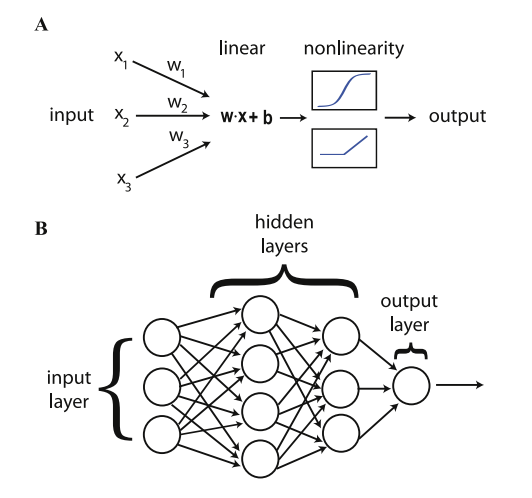
\includegraphics[width=10cm]{figures/basic_architecture.png}
%     \caption{$\textbf{(A)}$ The fundamental structure of neural networks comprises simplified nodes units that perform a linear operation to assign different weights to inputs, followed by a nonlinear activation function. $\textbf{(B)}$ These nodes units are organized into layers, where the output of one layer serves as the input to the subsequent layer, forming a hierarchical arrangement. \rednote{Add proper citation.}}
%     \label{fig:NN_basic_architecture}
% \end{figure}



% where $a$ is the output of the node, and is the value of the nodes activation function $f$ which has as input a weighted sum of signals $x_i, x_{i+1},...,x_n$ recieved by $n$ other nodes, multiplied with the weights $w_i, w_{i+1}, ..., w_{n}$ and added with biases $b_i, b_{i+1}, ..., b_{n}$. Biases, represented by $b_i$ for each node, provide an additional adjustment to the weighted sum, allowing the network to model biases in the data and play a crucial role in the overall flexibility of artificial neurons. The exact expression of $a$ varies depending on the type of nonlinearity that exists in the activation function applied to the input of each node. However, in almost all cases $a$ can be decomposed into a linear operation that weights the relative importance of the various inputs, and a nonlinear transformation $f(z)$. As seen in equation \ref{eq:neuron}, the linear tranformation commonly takes the form of a dot product with a set of node-specific weights followed by re-centering with a node-specific bias. A more convenient notation for the linear transformation $z^{i}$ then goes as follows:
%
% \begin{equation}
% z^{i} = \boldsymbol{w}^{(i)} \cdot \boldsymbol{x} + b^{(i)} = \mathbf{x}^T \cdot \mathbf{w}^{(i)} ,
% \label{eq:linear_transformation}
% \end{equation}
%
% where $\mathbf{x} = (1, \boldsymbol{x})$ and $\mathbf{w}^i = (b^{(i)}), \boldsymbol{w}^{(i)})$. The full input-output function can be expressed by incorporating this into the nonlinear activation function $f_i$, as expressed below:
% % TODO: f_i or a_i here?
%
% \begin{equation}
% a_i(\mathbf{x}) = f_i(z^{(i)}) .
% \label{eq:linear_transformation}
% \end{equation}


\section{Building a Feed-Forward Neural Network}
%The development of DiLoc started with a deliberate and cautious approach, focusing on simplicity without compromising on accuracy in tackling the inverse problem.
\rednote{Did not test other architectures?}
The feed-forward neural network was one of the first artificial neural network to be adopted and is yet today a wildly used algorithm within the domain of machine learning. As a natural starting point, we therefore adopted a fully connected, feed-forward neural network architecture for the purpose of solving the inverse problem. This approach eventually proved to be the most suitable framework among the ones tested. The fully connected feed-forward neural network is known as one of the simpler forms of neural networks, where information is processed in a unidirectional manner, flowing from the input nodes through the hidden layers and ultimately to the output nodes.



\subsection{Architecture}

% All inner parameters of the networks (weights and biases) are adjustable. Due to the layered structure of FNN the learning process is complicated, inefficient, and requires the activation functions of neurons to be differentiable. The training usually employ some form of gradient descent method, which is generally time-consuming and converges to local minima. Moreover some parameters, such as number of hidden neurons or learning algorithm parameters, have to be tuned manually.
% https://link.springer.com/chapter/10.1007/978-3-319-26227-7_6

In our initial testing phase, we tried different network configurations through an
iterative trial-and-error procedure. Different network architectures with various numbers of hidden layers and nodes were systematically examined. Ultimately, we settled on a model with roughly 300,000 trainable parameters which, after tweaking additional network attributes which will be elaborated upon later in this chapter, yielded promising results in terms of prediction accuracies.

The input layer is designed with 231 nodes, corresponding to the number of features in our data set, i.e. the number of recording electrodes for each sample. Subsequently, the network consists of five hidden layers, comprising 512, 256, 128, 64, and 32 nodes, respectively. Finally, the output layer holds an $x$-, $y$- and $z$-coordinate representing the predicted position of the dipole source. Figure \ref{fig:FCNN_architecture} visualizes the structure of the fully connected neural network.

\begin{figure}[!htb]
    \centering
    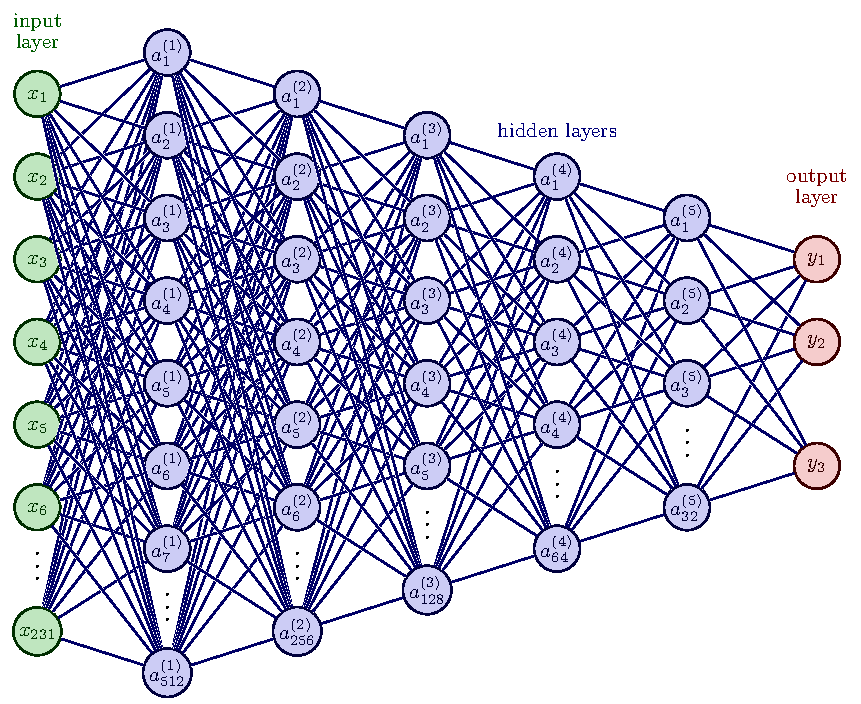
\includegraphics[width=\linewidth]{figures/FFNN_architecture.pdf}
    \caption{\textbf{Architecture of the fully connected Feed-Forward Neural Network}. The input layer comprises 231 electrode recording input values, and the network outputs predicted $x$-, $y$-, and $z$-coordinates of the dipole generating the EEG signal. The FCNN consists of five hidden layers. \\
    The visualization has been made with Latex, with code adapted from Neural Networks in TikZ with attribution to Izaak Neutelings and is licensed under the Creative Commons Attribution-ShareAlike 4.0 International License \cite{neutelings2021}.}
    \label{fig:FCNN_architecture}
\end{figure}



\subsection{Activation Functions}

Activation functions are fundamental components within the architecture of neural networks. Essentially, these functions introduce nonlinearity into the network's computations, thereby enabling the network to capture and model complex relationships within data \cite{sharma2017activation}. This property is essential because many real-world phenomena and data patterns exhibit inherent nonlinearity. Without activation functions, neural networks would essentially be linear regression models, limiting their ability to predict other relationships between inputs and outputs. In neural networks, activation functions are typically applied at every node within the hidden layers and sometimes at the output nodes in the final layer.
%In the context of solving the EEG inverse problem, where the EEG data contains intricate, nonlinear patterns, activation functions empower DiLoc to effectively model and learn from the EEG data structures.

Drawing inspiration from the behavior of biological neurons, activation functions can be understood as decision-makers within the artificial neural network, determining which information should be relayed to the next node. This process is analogous to the process in biophysics where the axon of one cell takes the output signal from the preceding cell and converts it into a format suitable for input to the next cell. Some activation functions can also be directly associated with biological phenomena like action potentials and spikes within neurons. Similar to how real neurons respond to incoming electrical signals, activation functions decide whether a node in a neural network should be activated or not based on the strength of the input it receives. If the input exceeds a certain threshold, the artificial neuron ``fires''; otherwise, it remains inactive \cite{analyticsvidhya_activationfunctions}.


\subsubsection{Rectified Linear Unit}
Within the input layer of the FCNN network, nodes utilize the \emph{Rectified Linear Units} (ReLU) activation function
defined as
\begin{equation}
  \text{ReLU}(x) = \begin{cases}
  x, & \text{if } x > 0 \\
  0, & \text{otherwise,}
\end{cases}
\label{eq:ReLU}
\end{equation}
and visually depicted in Figure \ref{fig:ReLU}.
ReLU closely resembles the behavior  of biological neurons. Specifically, it echoes the concept of the action potential: if a threshold is reached, the neuron fires; otherwise, the neuron remains inactive. Positive input values remain unchanged, while negative input values are suppressed by setting them to zero.
The widespread adoption of ReLU in neural networks can be attributed to its advantages in terms of computational speed, performance, and generalization capabilities.
\begin{figure}[ht]
    \centering
    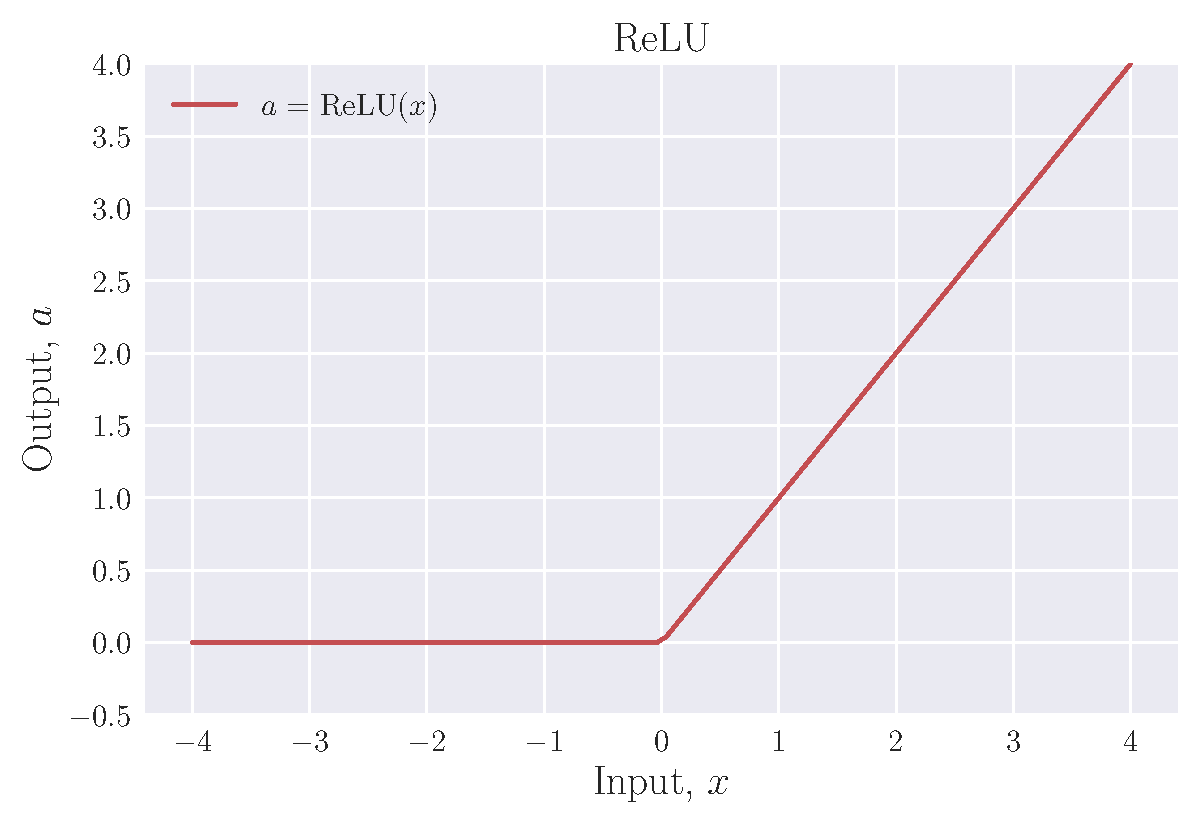
\includegraphics[width=\linewidth]{figures/ReLU.pdf}
    \caption{\textbf{Rectified Linear Unit (ReLU) Activation Function}: preserves positive input values \(x\) unchanged and enforces a transformation of negative input values to zero.}
    \label{fig:ReLU}
\end{figure}


\subsubsection{Hyperbolic Tangent}
For the hidden layers, we employed another activation function known as the \emph{Hyperbolic Tangent} (tanh) defined by
\begin{equation}
  \tanh(x) = \frac{e^x - e^{-x}}{e^x + e^{-x}},
\end{equation}
which is visualized in Figure \ref{fig:Tanh}.
This activation function smoothly compresses input values into the range between \(-1\) and 1, thereby preventing activations from becoming large, which could potentially cause problems during training.
While ReLU is known for its computational speed and simplicity, tanh has the possible advantage that it keeps all data flowing through the network during a forward pass. ReLU effectively removes the flow of information from some nodes through the network by clipping all negative values to zero. This could be a positive feature, but potentially also a problem causing some of the nodes to never be able to influence the output of the model, thereby decreasing its ability to learn.
\begin{figure}[ht]
    \centering
    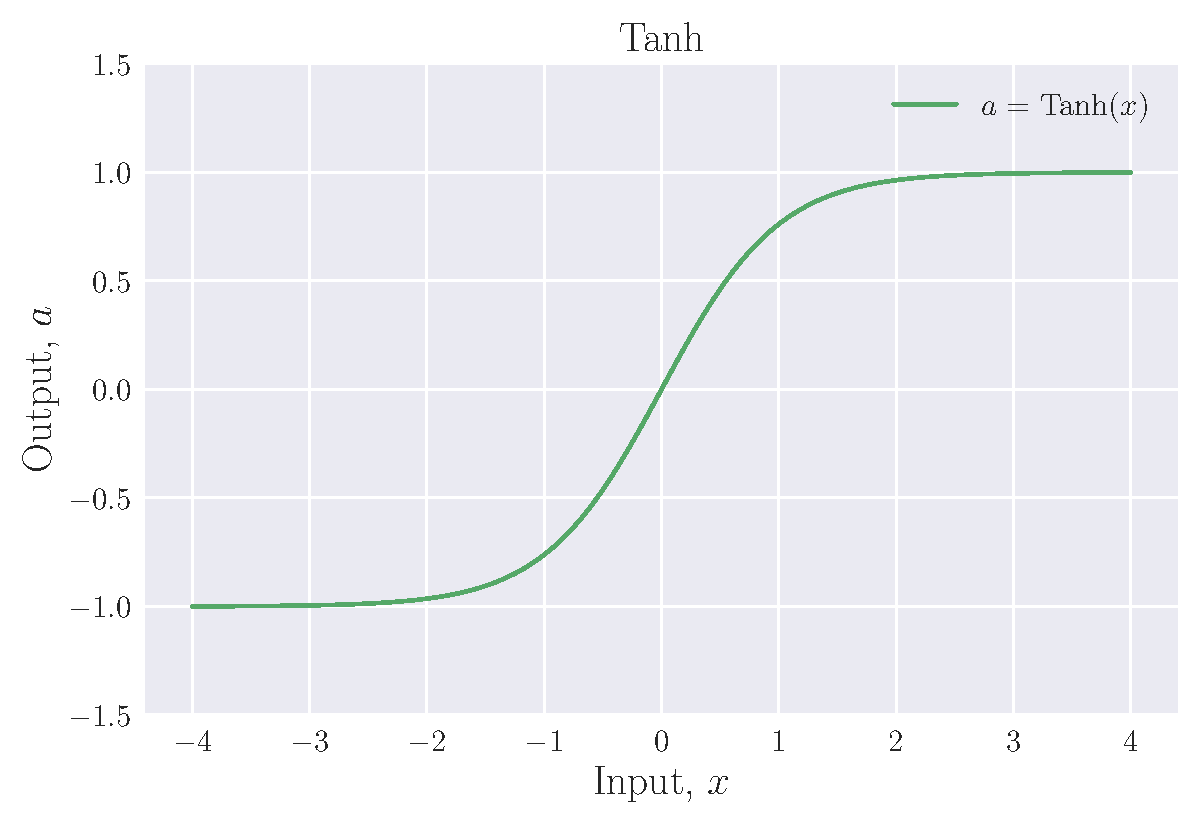
\includegraphics[width=\linewidth]{figures/Tanh.pdf}
    \caption{\textbf{Hyperbolic tangent activation function}: maps the input value $x$ into a continuous range between -1 and 1.}
    \label{fig:Tanh}
\end{figure}

%aim for the network to achieve a stable and effective learning process.
% tanh is continuous and differentiable at all points, that for reasons we will come back to is making it a suitable activation function for neural networks \rednote{Where do I come back to this?}.


\subsubsection{Linear Activation}

In our specific application, the target positions are the coordinates of current dipole sources, with values ranging from -70 to 70 mm for $x$, -58 to 78 mm for $y$, and -69 to 59 mm for $z$.
In the context of regression problems like ours, it is common practice to use linear activations -- which is simply the absence of any activation function at all -- in the output layer. We have done the same in our model, thus enabling it to output unbounded coordinate values.



\subsection{Initialization of Parameters}

% 231*512 + 512*256 + 256*128 + 128*64 + 64*32 + 32*3 + (512 + 256 + 128 + 64 + 32 + 3) = 293443

Neural networks train by fine-tuning their parameters \(\boldsymbol \theta\) to capture and adapt to intricate patterns within data. Weights and biases serve as the inner parameters of neural networks. The total number of parameters is equal to the sum of all connections between layers plus the total number of biases in every layer. In the architecture provided in Figure \ref{fig:FCNN_architecture}, our FCNN comprises just under 300,000 parameters.

The \emph{initialization} of weights and biases can significantly impact how quickly the model converges during training, and there exist several procedures commonly employed. In the FCNN we have used Xavier initialization, as this procedure is commonly paired with the tanh activation function, which is the one applied in our hidden layers. For every layer $l$, the weights $w^{(l)}$ are sampled from a normal distribution with mean \(\mu\) and variance \(\sigma^2\):
\begin{equation}
  w^{(l)} \sim \mathcal{N} \left( \mu=0, \sigma^2 = \frac{2}{N_{l-1} + N_l} \right).
\end{equation}
\(N_l\) denotes the number of neurons in layer \(l\).
\(N_l\) and \(N_{l - 1}\) are the number of rows and columns in \(w^{(l)}\) respectively.
The biases \(b^{(l)}\) are sampled uniformly between
\(- \sqrt{\frac{1}{N_{l - 1}}}\)
and
\(\sqrt{\frac{1}{N_{l - 1}}}\):
\begin{equation}
  b^{(l)} = \mathcal U \left( - \sqrt{\frac{1}{N_{l - 1}}}, \sqrt{\frac{1}{N_{l - 1}}} \right).
\end{equation}





\end{document}
